% Created by tikzDevice version 0.10.1 on 2016-06-26 23:06:37
% !TEX encoding = UTF-8 Unicode
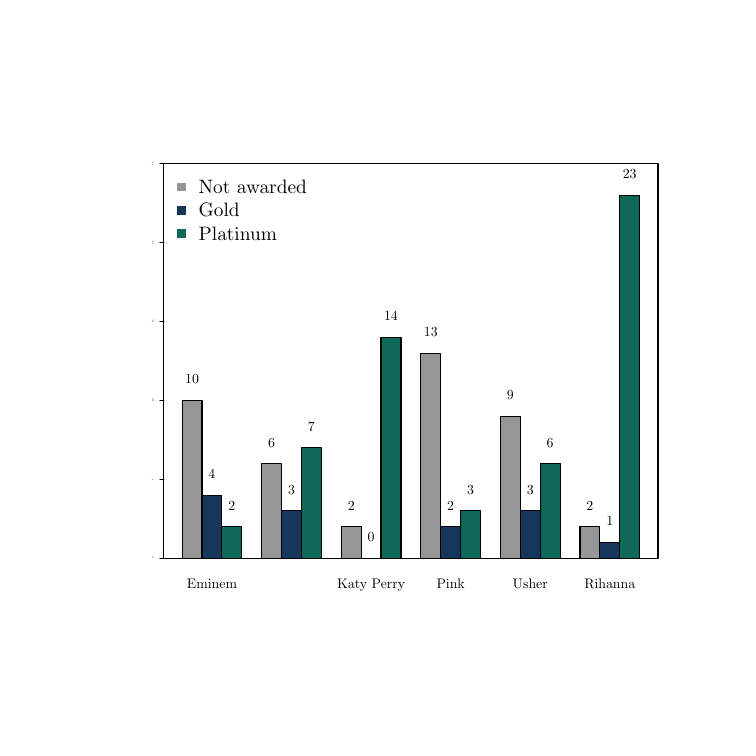
\begin{tikzpicture}[x=1pt,y=1pt]
\definecolor{fillColor}{RGB}{255,255,255}
\path[use as bounding box,fill=fillColor,fill opacity=0.00] (0,0) rectangle (252.94,252.94);
\begin{scope}
\path[clip] (  0.00,  0.00) rectangle (252.94,252.94);
\definecolor{drawColor}{RGB}{0,0,0}
\definecolor{fillColor}{gray}{0.59}

\path[draw=drawColor,line width= 0.4pt,line join=round,line cap=round,fill=fillColor] ( 55.81, 61.20) rectangle ( 63.00,118.22);
\definecolor{fillColor}{RGB}{22,54,92}

\path[draw=drawColor,line width= 0.4pt,line join=round,line cap=round,fill=fillColor] ( 63.00, 61.20) rectangle ( 70.19, 84.01);
\definecolor{fillColor}{RGB}{14,105,90}

\path[draw=drawColor,line width= 0.4pt,line join=round,line cap=round,fill=fillColor] ( 70.19, 61.20) rectangle ( 77.38, 72.60);
\definecolor{fillColor}{gray}{0.59}

\path[draw=drawColor,line width= 0.4pt,line join=round,line cap=round,fill=fillColor] ( 84.56, 61.20) rectangle ( 91.75, 95.41);
\definecolor{fillColor}{RGB}{22,54,92}

\path[draw=drawColor,line width= 0.4pt,line join=round,line cap=round,fill=fillColor] ( 91.75, 61.20) rectangle ( 98.94, 78.31);
\definecolor{fillColor}{RGB}{14,105,90}

\path[draw=drawColor,line width= 0.4pt,line join=round,line cap=round,fill=fillColor] ( 98.94, 61.20) rectangle (106.13,101.11);
\definecolor{fillColor}{gray}{0.59}

\path[draw=drawColor,line width= 0.4pt,line join=round,line cap=round,fill=fillColor] (113.32, 61.20) rectangle (120.50, 72.60);
\definecolor{fillColor}{RGB}{22,54,92}

\path[draw=drawColor,line width= 0.4pt,line join=round,line cap=round,fill=fillColor] (120.50, 61.20) rectangle (127.69, 61.20);
\definecolor{fillColor}{RGB}{14,105,90}

\path[draw=drawColor,line width= 0.4pt,line join=round,line cap=round,fill=fillColor] (127.69, 61.20) rectangle (134.88,141.03);
\definecolor{fillColor}{gray}{0.59}

\path[draw=drawColor,line width= 0.4pt,line join=round,line cap=round,fill=fillColor] (142.07, 61.20) rectangle (149.25,135.32);
\definecolor{fillColor}{RGB}{22,54,92}

\path[draw=drawColor,line width= 0.4pt,line join=round,line cap=round,fill=fillColor] (149.25, 61.20) rectangle (156.44, 72.60);
\definecolor{fillColor}{RGB}{14,105,90}

\path[draw=drawColor,line width= 0.4pt,line join=round,line cap=round,fill=fillColor] (156.44, 61.20) rectangle (163.63, 78.31);
\definecolor{fillColor}{gray}{0.59}

\path[draw=drawColor,line width= 0.4pt,line join=round,line cap=round,fill=fillColor] (170.82, 61.20) rectangle (178.01,112.52);
\definecolor{fillColor}{RGB}{22,54,92}

\path[draw=drawColor,line width= 0.4pt,line join=round,line cap=round,fill=fillColor] (178.01, 61.20) rectangle (185.19, 78.31);
\definecolor{fillColor}{RGB}{14,105,90}

\path[draw=drawColor,line width= 0.4pt,line join=round,line cap=round,fill=fillColor] (185.19, 61.20) rectangle (192.38, 95.41);
\definecolor{fillColor}{gray}{0.59}

\path[draw=drawColor,line width= 0.4pt,line join=round,line cap=round,fill=fillColor] (199.57, 61.20) rectangle (206.76, 72.60);
\definecolor{fillColor}{RGB}{22,54,92}

\path[draw=drawColor,line width= 0.4pt,line join=round,line cap=round,fill=fillColor] (206.76, 61.20) rectangle (213.94, 66.90);
\definecolor{fillColor}{RGB}{14,105,90}

\path[draw=drawColor,line width= 0.4pt,line join=round,line cap=round,fill=fillColor] (213.94, 61.20) rectangle (221.13,192.34);
\end{scope}
\begin{scope}
\path[clip] (  0.00,  0.00) rectangle (252.94,252.94);
\definecolor{drawColor}{RGB}{0,0,0}

\node[text=drawColor,anchor=base,inner sep=0pt, outer sep=0pt, scale=  0.50] at ( 66.59, 50.40) {Eminem};

\node[text=drawColor,anchor=base,inner sep=0pt, outer sep=0pt, scale=  0.50] at (124.10, 50.40) {Katy Perry};

\node[text=drawColor,anchor=base,inner sep=0pt, outer sep=0pt, scale=  0.50] at (152.85, 50.40) {Pink };

\node[text=drawColor,anchor=base,inner sep=0pt, outer sep=0pt, scale=  0.50] at (181.60, 50.40) {Usher };

\node[text=drawColor,anchor=base,inner sep=0pt, outer sep=0pt, scale=  0.50] at (210.35, 50.40) {Rihanna};

\path[draw=drawColor,line width= 0.4pt,line join=round,line cap=round] ( 49.20, 61.20) -- ( 49.20,203.75);

\path[draw=drawColor,line width= 0.4pt,line join=round,line cap=round] ( 49.20, 61.20) -- ( 47.77, 61.20);

\path[draw=drawColor,line width= 0.4pt,line join=round,line cap=round] ( 49.20, 89.71) -- ( 47.77, 89.71);

\path[draw=drawColor,line width= 0.4pt,line join=round,line cap=round] ( 49.20,118.22) -- ( 47.77,118.22);

\path[draw=drawColor,line width= 0.4pt,line join=round,line cap=round] ( 49.20,146.73) -- ( 47.77,146.73);

\path[draw=drawColor,line width= 0.4pt,line join=round,line cap=round] ( 49.20,175.24) -- ( 47.77,175.24);

\path[draw=drawColor,line width= 0.4pt,line join=round,line cap=round] ( 49.20,203.75) -- ( 47.77,203.75);

\node[text=drawColor,rotate= 90.00,anchor=base,inner sep=0pt, outer sep=0pt, scale=  0.10] at ( 45.60, 61.20) {0};

\node[text=drawColor,rotate= 90.00,anchor=base,inner sep=0pt, outer sep=0pt, scale=  0.10] at ( 45.60, 89.71) {5};

\node[text=drawColor,rotate= 90.00,anchor=base,inner sep=0pt, outer sep=0pt, scale=  0.10] at ( 45.60,118.22) {10};

\node[text=drawColor,rotate= 90.00,anchor=base,inner sep=0pt, outer sep=0pt, scale=  0.10] at ( 45.60,146.73) {15};

\node[text=drawColor,rotate= 90.00,anchor=base,inner sep=0pt, outer sep=0pt, scale=  0.10] at ( 45.60,175.24) {20};

\node[text=drawColor,rotate= 90.00,anchor=base,inner sep=0pt, outer sep=0pt, scale=  0.10] at ( 45.60,203.75) {25};
\end{scope}
\begin{scope}
\path[clip] ( 49.20, 61.20) rectangle (227.75,203.75);
\definecolor{drawColor}{RGB}{0,0,0}

\node[text=drawColor,anchor=base,inner sep=0pt, outer sep=0pt, scale=  0.50] at ( 59.41,124.22) {10};

\node[text=drawColor,anchor=base,inner sep=0pt, outer sep=0pt, scale=  0.50] at ( 66.59, 90.01) {4};

\node[text=drawColor,anchor=base,inner sep=0pt, outer sep=0pt, scale=  0.50] at ( 73.78, 78.60) {2};

\node[text=drawColor,anchor=base,inner sep=0pt, outer sep=0pt, scale=  0.50] at ( 88.16,101.41) {6};

\node[text=drawColor,anchor=base,inner sep=0pt, outer sep=0pt, scale=  0.50] at ( 95.35, 84.31) {3};

\node[text=drawColor,anchor=base,inner sep=0pt, outer sep=0pt, scale=  0.50] at (102.53,107.11) {7};

\node[text=drawColor,anchor=base,inner sep=0pt, outer sep=0pt, scale=  0.50] at (116.91, 78.60) {2};

\node[text=drawColor,anchor=base,inner sep=0pt, outer sep=0pt, scale=  0.50] at (124.10, 67.20) {0};

\node[text=drawColor,anchor=base,inner sep=0pt, outer sep=0pt, scale=  0.50] at (131.28,147.03) {14};

\node[text=drawColor,anchor=base,inner sep=0pt, outer sep=0pt, scale=  0.50] at (145.66,141.32) {13};

\node[text=drawColor,anchor=base,inner sep=0pt, outer sep=0pt, scale=  0.50] at (152.85, 78.60) {2};

\node[text=drawColor,anchor=base,inner sep=0pt, outer sep=0pt, scale=  0.50] at (160.04, 84.31) {3};

\node[text=drawColor,anchor=base,inner sep=0pt, outer sep=0pt, scale=  0.50] at (174.41,118.52) {9};

\node[text=drawColor,anchor=base,inner sep=0pt, outer sep=0pt, scale=  0.50] at (181.60, 84.31) {3};

\node[text=drawColor,anchor=base,inner sep=0pt, outer sep=0pt, scale=  0.50] at (188.79,101.41) {6};

\node[text=drawColor,anchor=base,inner sep=0pt, outer sep=0pt, scale=  0.50] at (203.16, 78.60) {2};

\node[text=drawColor,anchor=base,inner sep=0pt, outer sep=0pt, scale=  0.50] at (210.35, 72.90) {1};

\node[text=drawColor,anchor=base,inner sep=0pt, outer sep=0pt, scale=  0.50] at (217.54,198.34) {23};
\definecolor{fillColor}{gray}{0.59}

\path[fill=fillColor] ( 53.92,193.77) --
	( 57.07,193.77) --
	( 57.07,196.92) --
	( 53.92,196.92) --
	cycle;
\definecolor{fillColor}{RGB}{22,54,92}

\path[fill=fillColor] ( 53.92,185.37) --
	( 57.07,185.37) --
	( 57.07,188.52) --
	( 53.92,188.52) --
	cycle;
\definecolor{fillColor}{RGB}{14,105,90}

\path[fill=fillColor] ( 53.92,176.97) --
	( 57.07,176.97) --
	( 57.07,180.12) --
	( 53.92,180.12) --
	cycle;

\node[text=drawColor,anchor=base west,inner sep=0pt, outer sep=0pt, scale=  0.70] at ( 61.80,192.93) {Not awarded};

\node[text=drawColor,anchor=base west,inner sep=0pt, outer sep=0pt, scale=  0.70] at ( 61.80,184.53) {Gold};

\node[text=drawColor,anchor=base west,inner sep=0pt, outer sep=0pt, scale=  0.70] at ( 61.80,176.13) {Platinum};
\end{scope}
\begin{scope}
\path[clip] (  0.00,  0.00) rectangle (252.94,252.94);
\definecolor{drawColor}{RGB}{0,0,0}

\path[draw=drawColor,line width= 0.4pt,line join=round,line cap=round] ( 49.20, 61.20) --
	(227.75, 61.20) --
	(227.75,203.75) --
	( 49.20,203.75) --
	( 49.20, 61.20);
\end{scope}
\end{tikzpicture}
